\minitoc

\vfill

\clearpage

\section{\textsc{Feature baseline}}
    In order to detect such specific labels while guarantying a certain flexibility towards reference data, multiple modalities are necessary.
    The structure of the 3D model can be directly used to extract geometrical features.
    Dense depth information can be added, through for instance a \gls{acr::dsm}, so as to help detecting geometric defects that can be hardly discriminated otherwise (as in Figure~\ref{fig::fac_err}.(e)), in particular for the outer part of buildings. VHR optical images bring additional information (high frequencies and texture) that is particularly suited for inner defect detection.

    Since there is no comparable work that studies the previously defined errors, we propose a baseline for each modality.
    Attributes are kept simple so as to be used in most situations relying on generally available data. We avoid computing and comparing 3D lines~\parencite{michelin2013quality}, correlation scores~\parencite{boudet2006supervised} or any Structure-from-Motion (SfM) based metric~\parencite{kowdle2011active}.
    In addition of being very costly, these features are methodologically redundant with the 3D modeling techniques: they are vulnerable to the same defects.
    Conversely, evaluation metrics used in the 3D building reconstruction literature (\textit{e.g.}, \gls{acr::rmse}) are too weak for such a complex task.

    \subsection{\textsc{Geometric features}}
        The model facet set is denoted by $\mathsf{F}$.
        $\forall (f, g) \in \mathsf{F} \times \mathsf{F} \; f \sim g$ correspond to facets $f$ and $g$ being adjacent:
        \textit{i.e.}, they share a common edge. As the roof topology graph in~\parencite{verma20063d}, the input building model $\mathsf{M}$ can be seen as a facet (dual) graph:

        \begin{equation}
        	\label{eq::model_graph}
        	\mathsf{M} \triangleq \Big(\mathsf{F}, \mathsf{E} \triangleq \big\{ \{f, g\} \subset \mathsf{F} : f \sim g \big\} \Big).
        \end{equation}

        \begin{figure}[htbp]
            \centering
            \includestandalone[mode=buildnew, width=.75\textwidth]{figures/features/geometric_features}
            \caption{
                \label{fig::geometric_features}
                Computed geometric attributes represented on the dual graph, for facets $f$ and $g$.
                The green vector groups the node (facet) attributes while the blue one shows the edge features.
            }
        \end{figure}
        The dual graph is illustrated in Figure~\ref{fig::geometric_features}.
        For each facet $f \in \mathsf{F}$, we compute its degree (\textit{i.e.}, number of vertices; $d(f) \triangleq \vert\{v : v\text{ is a vertex of }f\}\vert$), its area $\mathscr{A}(f)$ and its circumference $\mathscr{C}(f)$.
        For each graph edge $e=\{f, g\} \in \mathsf{E}$, we look for the distance between facet centroids $\Vert \mathscr{G}(f) - \mathscr{G}(g) \Vert$ and the angle formed by their normals $\arccos(\vec{n}(f), \vec{n}(g))$.
        Statistical characteristics are then computed over building model facets using specific functions $S$, like a histogram:        

        \begin{equation}
        	S = S^p_{hist}: l \mapsto histogram(l, p),
        \end{equation}
        with $p$ standing for histogram parameters. A simpler option could be:
        \begin{equation}
            S = S_{synth}: l \mapsto \begin{bmatrix}
                \max(l)\\
                \min(l)\\
                \text{mean}(l)\\
                \text{median}(l)\\
                \sigma(l)
            \end{bmatrix},
        \end{equation}
        where:
        \begin{conditions}
            \sigma(l) & represents the standard deviation over a tuple $l$
        \end{conditions}

        These features are designed for general topological errors.
        For instance, over-segmentation may result in small facet areas and small angles between their normals.
        Conversely, an undersegmented facet would have a large area.
        Later on, the importance of these features will be discussed in details based on experimental results.
        
        Each building $\mathsf{M}$ can consequently be characterized by a geometric feature vector that accounts for its geometric characteristics:

        \begin{equation}
        	\label{eq::geom_feat}
            v_{geometric}(\mathsf{M}) = \begin{bmatrix}
            	S \Big(\big(d(f)\big)_{f \in \mathsf{F}}\Big)\\
                S \Big(\big(\mathscr{A}(f)\big)_{f \in \mathsf{F}}\Big)\\
                S \Big(\big(\mathscr{C}(f)\big)_{f \in \mathsf{F}}\Big)\\
                S \Big(\big( \vert\vert \mathscr{G}(f) - \mathscr{G}(g) \vert\vert \big)_{(f,g) \in \mathsf{E}}\Big)\\
                S\Big(\big( \arccos(\vec{n}(f) \cdot \vec{n}(g)) \big)_{(f,g) \in \mathsf{E}}\Big)
            \end{bmatrix}.
        \end{equation}
        Additionally to individual facet statistics, regularity is taken into account by looking into adjacent graph nodes as in~\parencite{zhou20102}.
        Such features express a limited  part of structural information.
        Taking this type of information into account would implicate graph comparisons which are not genuinely simple tasks to achieve.
        Since our objective is to build a baseline, this approach has not yet been considered.

    \subsection{\textsc{Height based features}}
        For this modality, raw depth information is provided by a \gls{acr::dsm} as a 2D height grid: $dsm \in \mathbb{R}^{w\times h}$\footnote{$w$ (\textit{resp.} h) is the grid width (\textit{resp.} height)}.
        It must have been produced around the same time of the 3D reconstruction so as to avoid temporal discrepancies.
        It is compared to the model height~\parencite{bredif20073d,zebedin2008fusion}.
        The latter is inferred from its facets plane equations.
        It is then rasterized into the image: $alt \in \mathbb{R}^{w\times h}$ at the same spatial resolution as $dsm$.
        Their difference generates a discrepancy map (Figure~\ref{fig::pipeline}.c).
        A baseline approach is proposed relying on the statistics of pixel values computed using the $S$ functions (Figure~\ref{fig::height_based_features}).

        \begin{equation}
            \label{eq::height_based_features}
            v_{height}(\mathsf{M}) = S\big( dsm - alt \big).
        \end{equation}
        \begin{figure}[H]
            \includestandalone[mode=buildnew,width=\textwidth]{figures/features/altimetric_features}
            \caption{
                \label{fig::height_based_features}
                Histogram height-based features computed from the \gls{acr::dsm} residuals.
                (a) \glspl{acr::dsm}.
                (b) Height maps extracted from the 3D model.
                (c) Difference between (a) and (b).
                The difference is transformed into a vector using a histogram (d).
            }
        \end{figure}
        Equation~\ref{eq::height_based_features} summarizes how building height-based features are computed. Different from a root mean square metric~\parencite{lafarge2012creating,poullis2013framework}, the histogram captures the discrepancy distribution, which is particularly helpful in detecting undersegmentation defects or geometric imprecision. However, as for the previous geometric attributes, the grid structure of information coming from the model is lost. Errors cannot be spatialized and linked to a specific facet.

    \subsection{\textsc{Image based features}}
        We aim to benefit from the high frequencies in Very High Spatial Resolution optical images. Building edges correspond to sharp discontinuities in images~\parencite{ortner2007building}. We verify this by comparing these edges to local gradients. We start by projecting building models on the orthorectified image $I$ (Figure~\ref{fig::radio}). For each facet, we isolate an edge $s$ (Figure~\ref{fig::seg_inter}). In an ideal setting, gradients computed at pixels $g$ that intersect $s$ need to be almost be collinear with its normal $\vec{n}(s)$. In consequence, applying the same statistics functions $S$, we compute the distribution of the cosine similarity between the local gradient and the normal all along that $s$:
        \begin{equation}
            \label{eq::corr_seg}
            \mathsf{D}_S(s, I) \triangleq S \bigg( \Big(\frac{\nabla I(g) \cdot \vec{n}(s)}{\Vert \nabla I(g)\Vert}\Big)_{g \in I \textrm{ and } g \cap s \neq \emptyset} \bigg).
        \end{equation}

        \begin{figure}[H]
            \begin{center}
                \floatbox{figure}{
                    \begin{subfloatrow}[2]
                        \ffigbox[\FBwidth]{
                            \caption{
                                Model facets (each represented by a specific color) are nadir projected onto the orthoimage.
                            }\label{fig::radio}
                            }			
                            {
                                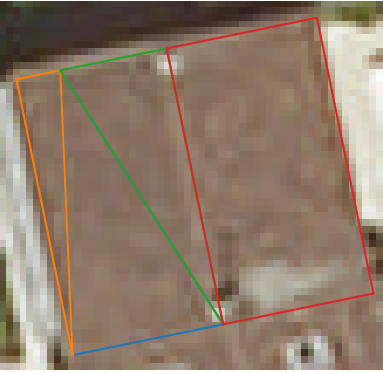
\includegraphics[width=.45\textwidth]{images/features/image/nadir_superposition}
                            }
                        \quad
                        \ffigbox[\FBwidth]{
                                \caption{Local gradients (in purple), on intersecting pixels (in green), are compared to the edge (in red) normal (in black).}\label{fig::seg_inter}
                            }
                            {\includestandalone[mode=buildnew, width=.45\textwidth]{figures/features/radiometric_features}
                        }
                    \end{subfloatrow}
                }{
                    \caption{Illustration of how features are derived from optical images.}\label{fig::image_based}
                }
            \end{center}
        \end{figure}

        Once the distribution is computed over a segment, it is stacked over all facet edges to define the distribution over projected facets. In the case of histograms $S_{hist}^p$ with the same parameters (and thus the same bins), it is equivalent to summing out the previous vectors $\mathsf{D}_{S_{hist}^p}(s, I)$ over edges $s$ from the projection $q(f)$ of the facet $f$. In order to take into account the variability of segment dimensions, this sum is normalized by segment lengths.
        \begin{equation}
            \label{eq::corr_fac}
            D_{S_{hist}^p}(f, I) \triangleq \sum_{s \in q(f)} \Vert s \Vert \cdot \mathsf{D}_{S_{hist}^p}(s, I).
        \end{equation}

        The same can be done over all facets of a building $\mathsf{M}$ (Equation~\ref{eq::corr_bul}). The weights are added in order to take into account the geometry heterogeneity. The gradient to normal comparison is similar to the 3D data fitting term formulated in~\parencite{li2016boxfitting}. Once again, the model structure is partially lost when simply summing histograms over all segments.
        \begin{equation}
            \label{eq::corr_bul}
            v_{image}(\mathsf{M}) = D_{S_{hist}^p}(\mathsf{M}, I) \triangleq \sum_{f \in \mathsf{F}} \mathscr{A}(q(f)) \cdot \mathsf{D}_{S_{hist}^p}(f, I).
        \end{equation}
        
        These image-based attributes are helpful for precision error detection. As example, facet imprecise borders can be detected as local gradients direction will be expected to differ greatly from the inaccurate edge. It can also be detrimental in under-segmentation detection as colors can change considerably from one facet or one building to another inducing an gradient orthogonal to edge normals.

    \section{\textsc{Classification process}}
        Two sources of flexibility are taken into account.
        First, the parametric nature of the taxonomy leads to a varying set of label.
        Secondly, the classifier should be able to handle the heterogeneity of the feature vector and must adapt to different input vectors types and sizes.

    \subsection{\textsc{Classification problems}}
        Both the classification problem nature and the label set are determined by the three previously defined taxonomy parameters (Table~\ref{tab::problems}).

        \begin{table}
            \begin{tabular}{c c c c}
                \toprule
                \textbf{\textit{finesse}} & \textbf{\gls{acr::elod}} & \textbf{exclusivity} & \textbf{Classification output}\\
                \midrule
                \scriptsize
                1 & --- & --- & Binary(Valid, Erroneous)\\
                2 & \gls{acr::lod}-1 & --- & Binary(Valid, Building error)\\
                2 & \gls{acr::lod}-2 & on & MultiClass(Valid, Building error, Facet error)\\
                2 & \gls{acr::lod}-2 & off & MultiLabel(Valid, Building error, Facet error)\\
                3 & \gls{acr::lod}-1 & on & MultiLabel(children(Binary(Valid, Building error)))\\
                3 & \gls{acr::lod}-2 & on & MultiLabel(children(MultiClass(Valid, Building error, Facet error)))\\
                3 & \gls{acr::lod}-1 & off & MultiLabel(children(Building error))\\
                3 & \gls{acr::lod}-2 & off & MultiLabel(children(Building error)$\cup$ children(Facet error))\\
                \bottomrule
            \end{tabular}
            \caption{
                \label{tab::problems} The summary of all possible classification problem types.
                children($error$) lists the children of $error$ from the taxonomy tree (Figure~\ref{fig::taxonomy}).
            }
        \end{table}
            
        \textbf{\textit{Finesse}} = 1 level corresponds to the standard binary classification problem: ` `Valid'' or ``Erroneous''.
        At \textit{finesse}=2, the \textbf{\gls{acr::elod}} can then take two values in the aerial reconstruction case: \gls{acr::lod}-1 or \gls{acr::lod}-2.
        If set at \gls{acr::lod}-1, it is a binary classification problem: ``Valid'' or ``Building error''.
        For \gls{acr::lod}-2, if the \textbf{exclusivity} is on, it will be a multi-class problem: ``Valid'', ``Building error'' or ``Facet errors''.
        If set off, it becomes a multi-label one with the same labels.
        At $\textit{finesse}=3$ level, if the \textbf{exclusivity} is on, it is a 2-stage classification problem.
        In the first stage, a multi-class task\footnote{It is binary in the spcial case \gls{acr::elod} = \gls{acr::lod}1, problem, like in the previous semantic degree.}
        predicts the error family, after which a second multi-label problem decides between the predicted error family children.
        If the \textbf{exclusivity} is off, it turns into  1-stage multi-label problem that predicts the existence of each atomic error corresponding to the chosen \gls{acr::elod}.

    \subsection{\textsc{Classifier choice}}
        The highly modular nature of the framework with multimodal features involving many parameters restricts the choice of classifiers.
        Random Forest classifiers~\parencite{breiman2001random,criminisi2013decision} are selected.
        They can manage a large number of features with different dynamics and coming from multiple modalities.
        Relying on their bagging property, a high number of trees ($1,000$ elements) is necessary to cover most of the feature space, while a limited tree depth ($4$) helps avoiding overfitting during training.
        It adapts to any of our classification paradigm: multi-class or multi-label.
        In the latter case, a one-vs-all approach is adopted in addition so as to address each label separately.

\section{\textsc{Richer features}}
    \subsection{\textsc{Graph classification}}
    \subsection{\textsc{Image classification}}
